\begin{frame}{\href{https://www.r-project.org/about.html}{What is R?} (R
Foundation 2017)}

``R is a language and environment for statistical computing and
graphics. It is a GNU project which is similar to the S language and
environment which was developed at Bell Laboratories (formerly AT\&T,
now Lucent Technologies) by John Chambers and colleagues. R can be
considered as a different implementation of S. There are some important
differences, but much code written for S runs unaltered under R.

R provides a wide variety of statistical (linear and nonlinear
modelling, classical statistical tests, time-series analysis,
classification, clustering, \ldots{}) and graphical techniques, and is
highly extensible. The S language is often the vehicle of choice for
research in statistical methodology, and R provides an Open Source route
to participation in that activity."

\end{frame}

\begin{frame}{(Some) Advantages of using R (from an R fanboy)}

\begin{itemize}
\tightlist
\item
  R is the most comprehensive statistical analysis software available.
\item
  R is a programming language developed by research and practicing
  statisticians for statisticians.
\item
  The graphical capabilities and options in R far surpasses the
  available graphical capabilities in other statistical packages.
\item
  R is free and open source licensed to The R Foundation for Statistical
  Computing under the GNU General Public License
\item
  R has a large community of users, developers, and bug-fixers. You can
  contribute to the development of R, too, by becoming an active member
  of the community.
\item
  R has over 10,000 packages available in CRAN and more available in
  bioconductor and Github repositories.
\item
  There are a lot of free books, websites, and coursewares available for
  learning R.
\end{itemize}

\end{frame}

\begin{frame}{(Some) Disadvantages of Using R}

\begin{itemize}
\tightlist
\item
  R has a steep learning curve (?)
\item
  Documentation is sometimes lacking
\item
  The quality of some packages is sometimes questionable
\item
  There is in general no one to complain to when something goes wrong
\item
  R's memory management sucks (?)
\end{itemize}

\end{frame}

\begin{frame}{\href{https://www.datasciencecentral.com/profiles/blogs/list-of-companies-using-r}{Who
Uses R?} (Bhalla 2017)}

\begin{itemize}
\tightlist
\item
  Facebook - For behavior analysis related to status updates and profile
  pictures.
\item
  Google - For advertising effectiveness and economic forecasting.
\item
  Twitter - For data visualization and semantic clustering
\item
  Microsoft - Acquired Revolution R company and use it for a variety of
  purposes.
\item
  Uber - For statistical analysis
\item
  Airbnb - Scale data science.
\item
  IBM - Joined R Consortium Group
\item
  ANZ - For credit risk modeling
\end{itemize}

\end{frame}

\begin{frame}{Why use R?}

\begin{itemize}
\tightlist
\item
  It is free (and open source)!
\item
  R is the most popular tool for analytics/data science (Piatetsky
  2016).
\item
  Ranked 5th in most popular software based on number of job offerings:
  SQL, Python, Java, Hadoop, R, C/C++/C\#, SAS, Apache Spark, Tableau,
  Apache Hive (Muenchen 2017)
\item
  R has surpassed SAS in scholarly use--but still way behind SPSS
  (Muenchen 2016)
\end{itemize}

\end{frame}

\begin{frame}{Is ``R also for Filipino Researchers''?}

Yes.

\end{frame}

\begin{frame}{I have no experience with coding so R frightens me.}

\begin{itemize}
\tightlist
\item
  You use Microsoft Excel, right?
\end{itemize}

\end{frame}

\begin{frame}{Why use Rstudio with R?}

\begin{center}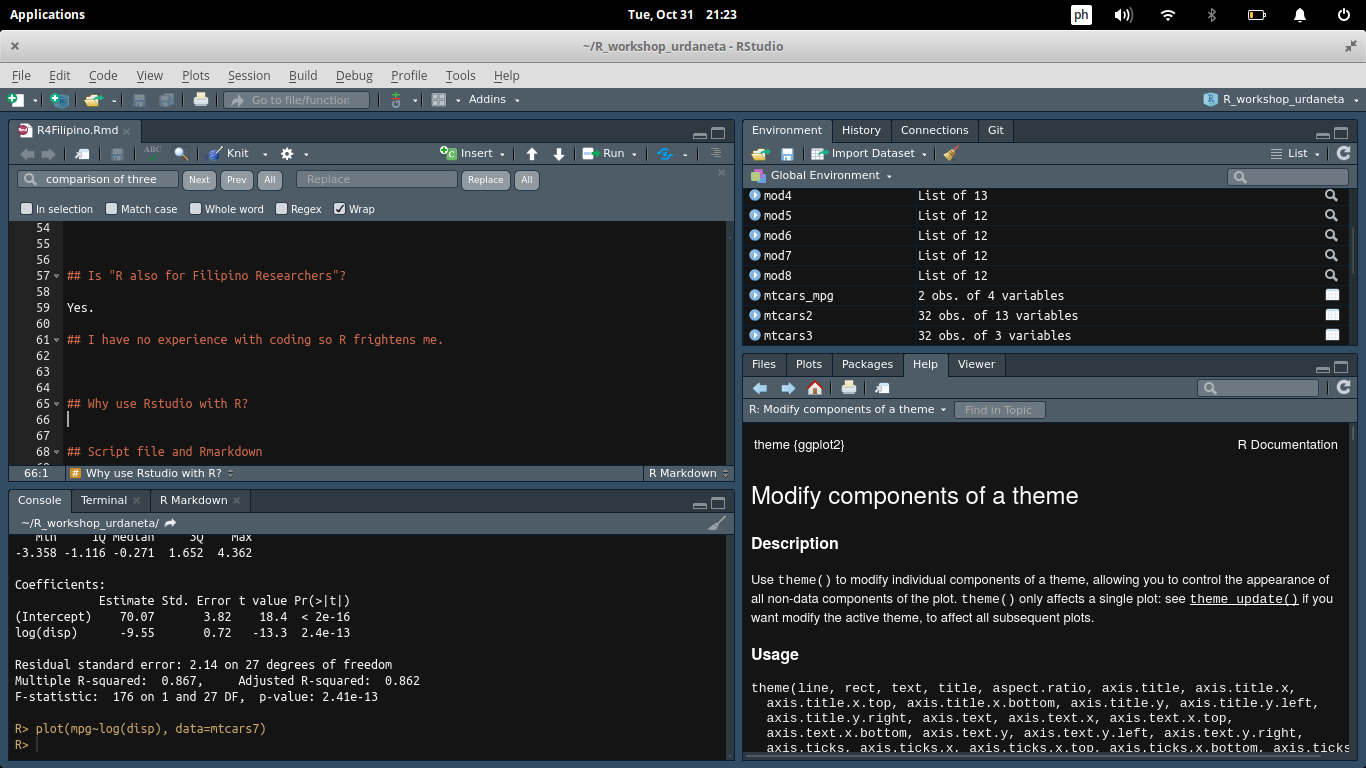
\includegraphics[width=900]{./img/Rmarkdown} \end{center}

\end{frame}

\begin{frame}[fragile]{Let's load the required packages first}

\begin{Shaded}
\begin{Highlighting}[]
\KeywordTok{library}\NormalTok{(tidyverse)}
\KeywordTok{library}\NormalTok{(agricolae)}
\end{Highlighting}
\end{Shaded}

\end{frame}

\begin{frame}[fragile]{Introducing the \texttt{mtcars\ data\ set}}

\begin{Shaded}
\begin{Highlighting}[]
\NormalTok{?mtcars}
\KeywordTok{write.csv}\NormalTok{(mtcars, }\StringTok{"mtcars.csv"}\NormalTok{)}
\end{Highlighting}
\end{Shaded}

\end{frame}

\begin{frame}[fragile]{Using different ways to load data set into R}

\begin{itemize}
\tightlist
\item
  Using the R console
\end{itemize}

\begin{Shaded}
\begin{Highlighting}[]
\NormalTok{mt1 <-}\StringTok{ }\KeywordTok{read.table}\NormalTok{(}\StringTok{"mtcars.csv"}\NormalTok{, }\DataTypeTok{sep =} \StringTok{","}\NormalTok{, }\DataTypeTok{header=}\OtherTok{TRUE}\NormalTok{)}
\NormalTok{mtcars2 <-}\StringTok{ }\KeywordTok{read.csv}\NormalTok{(}\StringTok{"mtcars.csv"}\NormalTok{)}
\NormalTok{mt3 <-}\StringTok{ }\KeywordTok{read_csv}\NormalTok{(}\StringTok{"mtcars.csv"}\NormalTok{)}
\NormalTok{mt4 <-}\StringTok{ }\NormalTok{data.table}\OperatorTok{::}\KeywordTok{fread}\NormalTok{(}\StringTok{"mtcars.csv"}\NormalTok{)}
\end{Highlighting}
\end{Shaded}

\begin{itemize}
\tightlist
\item
  From Rstudio, click \texttt{File\ \textgreater{}\ Import\ Dataset}.
\end{itemize}

\end{frame}

\begin{frame}{Linear Model for comparing the means of two groups}

\begin{block}{Means Model}

\[y_{ij} = \mu_i + \varepsilon_{ij},\, i = 1,2\]

\begin{itemize}
\tightlist
\item
  \(H_0: \mu_1 = \mu_2\)
\item
  \(H_a: \mu_1\neq\mu_2\)
\end{itemize}

\end{block}

\end{frame}

\begin{frame}[fragile]{Linear Model for comparing the means of two
groups}

\begin{block}{Effects Model}

\[y_{ij} = \mu + \alpha_i + \varepsilon_{ij},\, i = 1,2\]

where:

\begin{itemize}
\tightlist
\item
  \(y_{ij}=\) is the \(j\)th value of \texttt{mpg} in the \(i\)th group
  of \texttt{am}
\item
  \(\mu=\) mean of \(Y\)
\item
  \(\alpha_i = \) effect of the \(i\)th group of \texttt{am} on
  \texttt{mpg}
\item
  \(\varepsilon=\) the random error due to the \(j\)th value of
  \texttt{mpg} in the \(i\)th value of \texttt{am}
\end{itemize}

\end{block}

\begin{block}{Hypotheses}

\begin{itemize}
\tightlist
\item
  \(H_0: \alpha_1 = \alpha_2\)
\item
  \(H_a: \alpha_1\neq\alpha_2\)
\end{itemize}

\end{block}

\end{frame}

\begin{frame}{A research question: Is there a difference in milleage for
automatic and manual cars?}

\begin{itemize}
\item
  \(H_a: \alpha_1=\alpha_2=0\) (or \(\mu_1=\mu_2\)) The milleage per
  gallon differ based on transmission type of the car.
\item
  \(H_0: \alpha_1\neq\alpha_2\) (or \(\mu_1\neq\mu_2\)) The milleage per
  gallon do not differ based on transmission type of the car.
\end{itemize}

\end{frame}

\begin{frame}[fragile]{A research question: Is there a difference in
milleage for automatic and manual cars?}

\begin{Shaded}
\begin{Highlighting}[]
\KeywordTok{table}\NormalTok{(mtcars}\OperatorTok{$}\NormalTok{am)}
\end{Highlighting}
\end{Shaded}

\begin{verbatim}

 0  1 
19 13 
\end{verbatim}

\begin{Shaded}
\begin{Highlighting}[]
\KeywordTok{aggregate}\NormalTok{(mtcars}\OperatorTok{$}\NormalTok{mpg, }\DataTypeTok{by =} \KeywordTok{list}\NormalTok{(mtcars}\OperatorTok{$}\NormalTok{am), }\DataTypeTok{FUN=}\StringTok{"mean"}\NormalTok{)}
\end{Highlighting}
\end{Shaded}

\begin{verbatim}
  Group.1     x
1       0 17.15
2       1 24.39
\end{verbatim}

\begin{Shaded}
\begin{Highlighting}[]
\KeywordTok{aggregate}\NormalTok{(mtcars}\OperatorTok{$}\NormalTok{mpg, }\DataTypeTok{by =} \KeywordTok{list}\NormalTok{(mtcars}\OperatorTok{$}\NormalTok{am), }\DataTypeTok{FUN=}\StringTok{"var"}\NormalTok{)}
\end{Highlighting}
\end{Shaded}

\begin{verbatim}
  Group.1     x
1       0 14.70
2       1 38.03
\end{verbatim}

\end{frame}

\begin{frame}[fragile]{A research question: Is there a difference in
milleage for automatic and manual cars?}

\begin{Shaded}
\begin{Highlighting}[]
\NormalTok{mtcars_mpg <-}\StringTok{ }\NormalTok{mtcars }\OperatorTok
\StringTok{  }\KeywordTok{group_by}\NormalTok{(am) }\OperatorTok
\StringTok{  }\KeywordTok{summarise}\NormalTok{(}
    \DataTypeTok{mean_mpg =} \KeywordTok{mean}\NormalTok{(mpg),}
    \DataTypeTok{var_mpg =} \KeywordTok{var}\NormalTok{(mpg), }
    \DataTypeTok{n =} \KeywordTok{n}\NormalTok{()}
\NormalTok{  )}
\NormalTok{mtcars_mpg}
\end{Highlighting}
\end{Shaded}

\begin{verbatim}
# A tibble: 2 x 4
     am mean_mpg var_mpg     n
  <dbl>    <dbl>   <dbl> <int>
1     0    17.15   14.70    19
2     1    24.39   38.03    13
\end{verbatim}

\end{frame}

\begin{frame}[fragile]{Continuation of Eploratory Data Analysis}

\begin{Shaded}
\begin{Highlighting}[]
\KeywordTok{boxplot}\NormalTok{(mpg}\OperatorTok{~}\NormalTok{am, }\DataTypeTok{data =}\NormalTok{ mtcars)}
\end{Highlighting}
\end{Shaded}

\begin{center}\includegraphics[width=350]{R4Filipino_files/figure-beamer/unnamed-chunk-9-1} \end{center}

\end{frame}

\begin{frame}[fragile]{Changing the labels of a plot; creating a new
variable in a data set (\texttt{data.frame})}

Let us put some labels for the levels of \texttt{am}.

\begin{Shaded}
\begin{Highlighting}[]
\NormalTok{mtcars2}\OperatorTok{$}\NormalTok{amf <-}\StringTok{ }\KeywordTok{factor}\NormalTok{(mtcars2}\OperatorTok{$}\NormalTok{am, }\DataTypeTok{levels =} \KeywordTok{c}\NormalTok{(}\DecValTok{0}\NormalTok{,}\DecValTok{1}\NormalTok{), }\DataTypeTok{labels =} \KeywordTok{c}\NormalTok{(}\StringTok{"auto"}\NormalTok{, }\StringTok{"manual"}\NormalTok{))}
\KeywordTok{boxplot}\NormalTok{(mpg}\OperatorTok{~}\NormalTok{amf, }\DataTypeTok{data=}\NormalTok{mtcars2)}
\end{Highlighting}
\end{Shaded}

\begin{center}\includegraphics[width=350]{R4Filipino_files/figure-beamer/unnamed-chunk-10-1} \end{center}

\end{frame}

\begin{frame}[fragile]{Changing the x and y labels and putting a title}

Let us put some labels for the levels of \texttt{am}.

\begin{Shaded}
\begin{Highlighting}[]
\KeywordTok{boxplot}\NormalTok{(mpg}\OperatorTok{~}\NormalTok{amf, }\DataTypeTok{data=}\NormalTok{mtcars2, }
        \DataTypeTok{main =} \StringTok{"Boxplots of miles per gallon according to transmission type"}\NormalTok{,}
        \DataTypeTok{xlab =} \StringTok{"Transmission type"}\NormalTok{,}
        \DataTypeTok{ylab =} \StringTok{"Miles per gallon"}\NormalTok{)}
\end{Highlighting}
\end{Shaded}

\begin{center}\includegraphics[width=350]{R4Filipino_files/figure-beamer/unnamed-chunk-11-1} \end{center}

\end{frame}

\begin{frame}[fragile]{Changing the range of values in the \(y\)-axis}

Let us start the boxplot at 0.

\begin{Shaded}
\begin{Highlighting}[]
\KeywordTok{boxplot}\NormalTok{(mpg}\OperatorTok{~}\NormalTok{amf, }\DataTypeTok{data=}\NormalTok{mtcars2, }
        \DataTypeTok{main =} \StringTok{"Boxplots of miles per gallon according to transmission type"}\NormalTok{,}
        \DataTypeTok{xlab =} \StringTok{"Transmission type"}\NormalTok{,}
        \DataTypeTok{ylab =} \StringTok{"Miles per gallon"}\NormalTok{,}
        \DataTypeTok{ylim =} \KeywordTok{c}\NormalTok{(}\DecValTok{0}\NormalTok{,}\DecValTok{35}\NormalTok{))}
\end{Highlighting}
\end{Shaded}

\begin{center}\includegraphics[width=350]{R4Filipino_files/figure-beamer/unnamed-chunk-12-1} \end{center}

\end{frame}

\begin{frame}[fragile]{Plotting with \texttt{ggplot2}}

\begin{Shaded}
\begin{Highlighting}[]
\KeywordTok{ggplot}\NormalTok{(mtcars2, }\KeywordTok{aes}\NormalTok{(}\DataTypeTok{x =}\NormalTok{ amf, }\DataTypeTok{y =}\NormalTok{ mpg)) }\OperatorTok{+}\StringTok{ }\KeywordTok{geom_boxplot}\NormalTok{() }\OperatorTok{+}\StringTok{ }\KeywordTok{ylim}\NormalTok{(}\DecValTok{0}\NormalTok{,}\DecValTok{35}\NormalTok{)}
\end{Highlighting}
\end{Shaded}

\begin{center}\includegraphics[width=350]{R4Filipino_files/figure-beamer/unnamed-chunk-13-1} \end{center}

\begin{Shaded}
\begin{Highlighting}[]
\CommentTok{# What is the difference?}
\KeywordTok{ggplot}\NormalTok{(mtcars2, }\KeywordTok{aes}\NormalTok{(}\DataTypeTok{x =}\NormalTok{ amf, }\DataTypeTok{y =}\NormalTok{ mpg)) }\OperatorTok{+}\StringTok{ }\KeywordTok{geom_boxplot}\NormalTok{() }\OperatorTok{+}\StringTok{ }\KeywordTok{coord_cartesian}\NormalTok{(}\DataTypeTok{ylim =} \KeywordTok{c}\NormalTok{(}\DecValTok{0}\NormalTok{,}\DecValTok{35}\NormalTok{)) }
\end{Highlighting}
\end{Shaded}

\end{frame}

\begin{frame}[fragile]{ggplot2 uses the language of graphics}

\begin{Shaded}
\begin{Highlighting}[]
\NormalTok{p <-}\StringTok{ }\KeywordTok{ggplot}\NormalTok{(mtcars2, }\KeywordTok{aes}\NormalTok{(}\DataTypeTok{x =}\NormalTok{ amf, }\DataTypeTok{y =}\NormalTok{ mpg)) }\OperatorTok{+}\StringTok{ }
\StringTok{  }\KeywordTok{geom_boxplot}\NormalTok{() }\OperatorTok{+}\StringTok{ }
\StringTok{  }\KeywordTok{xlab}\NormalTok{(}\StringTok{"Transmission type"}\NormalTok{) }\OperatorTok{+}\StringTok{ }
\StringTok{  }\KeywordTok{ylab}\NormalTok{(}\StringTok{"Miles per gallon"}\NormalTok{) }
\NormalTok{p}
\end{Highlighting}
\end{Shaded}

\begin{center}\includegraphics[width=350]{R4Filipino_files/figure-beamer/unnamed-chunk-15-1} \end{center}

\end{frame}

\begin{frame}{A review of t test}

What are the assumptions of the independent samples t test?

\begin{enumerate}
\def\labelenumi{\arabic{enumi}.}
\tightlist
\item
  Dependent variable should be measured on a continuous scale (interval
  or ratio level)
\item
  Independent variable consist of two categorical, independet groups
\item
  Observations are independent of each other
\item
  No significant outliers
\item
  Dependent variable should be (approximately) normally distributed for
  each group of the independent variable
\item
  Variances should be homogenous
\end{enumerate}

\end{frame}

\begin{frame}{Applying the assumptions}

\begin{enumerate}
\def\labelenumi{\arabic{enumi}.}
\tightlist
\item
  What is the independent variable? What is the independent variable?
\item
  Is the dependent variable measured on a continuous scale?
\item
  Does the independent variable consist of two categorical, independent
  groups?
\item
  Are observations independent of each other?
\item
  Are there no significant outliers?
\item
  Is the dependent variable normally distributed for each group of the
  independent variable?
\item
  Are the variances homogenous?
\end{enumerate}

\end{frame}

\begin{frame}[fragile]{Normality for each group of the independent
variable}

\begin{Shaded}
\begin{Highlighting}[]
\KeywordTok{ggplot}\NormalTok{(mtcars2, }\KeywordTok{aes}\NormalTok{(}\DataTypeTok{x =}\NormalTok{ mpg, }\DataTypeTok{fill =}\NormalTok{ amf)) }\OperatorTok{+}\StringTok{ }\KeywordTok{geom_histogram}\NormalTok{(}\DataTypeTok{bins =} \DecValTok{5}\NormalTok{) }\OperatorTok{+}\StringTok{ }\KeywordTok{facet_wrap}\NormalTok{(}\OperatorTok{~}\NormalTok{amf, }\DataTypeTok{scales =} \StringTok{"free_x"}\NormalTok{)}
\end{Highlighting}
\end{Shaded}

\begin{center}\includegraphics[width=500]{R4Filipino_files/figure-beamer/unnamed-chunk-16-1} \end{center}

\end{frame}

\begin{frame}[fragile]{Homogeneity of variance}

\begin{Shaded}
\begin{Highlighting}[]
\NormalTok{p}
\end{Highlighting}
\end{Shaded}

\begin{center}\includegraphics[width=350]{R4Filipino_files/figure-beamer/unnamed-chunk-17-1} \end{center}

\end{frame}

\begin{frame}[fragile]{Homogeneity of variance (cont\ldots{})}

\begin{Shaded}
\begin{Highlighting}[]
\KeywordTok{var.test}\NormalTok{(mpg}\OperatorTok{~}\NormalTok{amf, }\DataTypeTok{data=}\NormalTok{mtcars2)}
\end{Highlighting}
\end{Shaded}

\begin{verbatim}

    F test to compare two variances

data:  mpg by amf
F = 0.39, num df = 18, denom df = 12, p-value = 0.07
alternative hypothesis: true ratio of variances is not equal to 1
95 percent confidence interval:
 0.1244 1.0703
sample estimates:
ratio of variances 
            0.3866 
\end{verbatim}

\end{frame}

\begin{frame}[fragile]{t test results}

\begin{Shaded}
\begin{Highlighting}[]
\NormalTok{(t1 <-}\StringTok{ }\KeywordTok{t.test}\NormalTok{(mpg }\OperatorTok{~}\StringTok{ }\NormalTok{amf, }\DataTypeTok{data =}\NormalTok{ mtcars2))}
\end{Highlighting}
\end{Shaded}

\begin{verbatim}

    Welch Two Sample t-test

data:  mpg by amf
t = -3.8, df = 18, p-value = 0.001
alternative hypothesis: true difference in means is not equal to 0
95 percent confidence interval:
 -11.28  -3.21
sample estimates:
  mean in group auto mean in group manual 
               17.15                24.39 
\end{verbatim}

\end{frame}

\begin{frame}[fragile]{How to use \texttt{t.test}?}

\begin{Shaded}
\begin{Highlighting}[]
\NormalTok{?t.test}
\end{Highlighting}
\end{Shaded}

\end{frame}

\begin{frame}[fragile]{How about independent samples t test?}

\begin{Shaded}
\begin{Highlighting}[]
\NormalTok{(t2 <-}\StringTok{ }\KeywordTok{t.test}\NormalTok{(mpg}\OperatorTok{~}\NormalTok{amf, }\DataTypeTok{data=}\NormalTok{mtcars2, }\DataTypeTok{var.equal=}\OtherTok{TRUE}\NormalTok{))}
\end{Highlighting}
\end{Shaded}

\begin{verbatim}

    Two Sample t-test

data:  mpg by amf
t = -4.1, df = 30, p-value = 3e-04
alternative hypothesis: true difference in means is not equal to 0
95 percent confidence interval:
 -10.848  -3.642
sample estimates:
  mean in group auto mean in group manual 
               17.15                24.39 
\end{verbatim}

\end{frame}

\begin{frame}[fragile]{Non-parametric alternative}

\begin{Shaded}
\begin{Highlighting}[]
\NormalTok{(w <-}\StringTok{ }\KeywordTok{wilcox.test}\NormalTok{(mpg }\OperatorTok{~}\StringTok{ }\NormalTok{amf, }\DataTypeTok{data =}\NormalTok{ mtcars2, }\DataTypeTok{conf.int =} \OtherTok{TRUE}\NormalTok{))}
\end{Highlighting}
\end{Shaded}

\begin{verbatim}
Warning in wilcox.test.default(x = c(21.4, 18.7, 18.1, 14.3, 24.4, 22.8, :
cannot compute exact p-value with ties
\end{verbatim}

\begin{verbatim}
Warning in wilcox.test.default(x = c(21.4, 18.7, 18.1, 14.3, 24.4, 22.8, :
cannot compute exact confidence intervals with ties
\end{verbatim}

\begin{verbatim}

    Wilcoxon rank sum test with continuity correction

data:  mpg by amf
W = 42, p-value = 0.002
alternative hypothesis: true location shift is not equal to 0
95 percent confidence interval:
 -11.7  -2.9
sample estimates:
difference in location 
                  -6.8 
\end{verbatim}

\end{frame}

\begin{frame}[fragile]{Confidence intervals}

\begin{Shaded}
\begin{Highlighting}[]
\NormalTok{t1}\OperatorTok{$}\NormalTok{conf.int}
\end{Highlighting}
\end{Shaded}

\begin{verbatim}
[1] -11.28  -3.21
attr(,"conf.level")
[1] 0.95
\end{verbatim}

\begin{Shaded}
\begin{Highlighting}[]
\NormalTok{t2}\OperatorTok{$}\NormalTok{conf.int}
\end{Highlighting}
\end{Shaded}

\begin{verbatim}
[1] -10.848  -3.642
attr(,"conf.level")
[1] 0.95
\end{verbatim}

\begin{Shaded}
\begin{Highlighting}[]
\NormalTok{w}\OperatorTok{$}\NormalTok{conf.int}
\end{Highlighting}
\end{Shaded}

\begin{verbatim}
[1] -11.7  -2.9
attr(,"conf.level")
[1] 0.95
\end{verbatim}

\end{frame}

\begin{frame}[fragile]{Determining other values from the tests}

\begin{Shaded}
\begin{Highlighting}[]
\KeywordTok{names}\NormalTok{(t1)}
\end{Highlighting}
\end{Shaded}

\begin{verbatim}
[1] "statistic"   "parameter"   "p.value"     "conf.int"    "estimate"   
[6] "null.value"  "alternative" "method"      "data.name"  
\end{verbatim}

\end{frame}

\begin{frame}{Conclusion of comparison of milleage according to
transmission type}

The milleage per gallon differ between manual and automatic
tramission-type vehicles by about 7.24 miles per gallon at \(0.05\)
significance level (or 95\% confidence level).

\end{frame}

\begin{frame}[fragile]{When to use one-tailed t test}

\begin{Shaded}
\begin{Highlighting}[]
\NormalTok{?t.test}
\end{Highlighting}
\end{Shaded}

\begin{Shaded}
\begin{Highlighting}[]
\NormalTok{(t3 <-}\StringTok{ }\KeywordTok{t.test}\NormalTok{(mpg }\OperatorTok{~}\StringTok{ }\NormalTok{amf, }\DataTypeTok{data =}\NormalTok{ mtcars2, }\DataTypeTok{alternative =} \StringTok{"less"}\NormalTok{))}
\end{Highlighting}
\end{Shaded}

\begin{verbatim}

    Welch Two Sample t-test

data:  mpg by amf
t = -3.8, df = 18, p-value = 7e-04
alternative hypothesis: true difference in means is less than 0
95 percent confidence interval:
   -Inf -3.913
sample estimates:
  mean in group auto mean in group manual 
               17.15                24.39 
\end{verbatim}

\begin{Shaded}
\begin{Highlighting}[]
\NormalTok{t3 }\OperatorTok\StringTok{ }\NormalTok{broom}\OperatorTok{::}\KeywordTok{tidy}\NormalTok{()}
\end{Highlighting}
\end{Shaded}

\begin{verbatim}
  estimate estimate1 estimate2 statistic   p.value parameter conf.low
1   -7.245     17.15     24.39    -3.767 0.0006868     18.33     -Inf
  conf.high                  method alternative
1    -3.913 Welch Two Sample t-test        less
\end{verbatim}

\end{frame}

\begin{frame}[fragile]{Comparison of the means of three groups}

\begin{Shaded}
\begin{Highlighting}[]
\KeywordTok{table}\NormalTok{(mtcars2}\OperatorTok{$}\NormalTok{cyl)}
\end{Highlighting}
\end{Shaded}

\begin{verbatim}

 4  6  8 
11  7 14 
\end{verbatim}

\begin{Shaded}
\begin{Highlighting}[]
\NormalTok{mtcars3 <-}\StringTok{ }\NormalTok{mtcars2 }\OperatorTok\StringTok{ }\KeywordTok{select}\NormalTok{(mpg, cyl)}
\KeywordTok{head}\NormalTok{(mtcars3)}
\end{Highlighting}
\end{Shaded}

\begin{verbatim}
   mpg cyl
1 21.0   6
2 21.0   6
3 22.8   4
4 21.4   6
5 18.7   8
6 18.1   6
\end{verbatim}

\end{frame}

\begin{frame}[fragile]{Linear Model for the problem of comparing three
means}

\[ y_{ij} = \mu + \alpha_i + \varepsilon_{ij},\, i = 1, 2, 3\] where:

\begin{itemize}
\tightlist
\item
  \(y_{ij}=\) is the \(j\)th value of \texttt{mpg} in the \(i\)th group
  of \texttt{cyl}
\item
  \(\mu=\) mean of \(Y\)
\item
  \(\alpha_i = \) effect of the \(i\)th group of \texttt{cyl} on
  \texttt{mpg}
\item
  \(\varepsilon=\) the random error due to the \(j\)th value of
  \texttt{mpg} in the \(i\)th value of \texttt{cyl}
\end{itemize}

\begin{block}{Hypotheses}

\begin{itemize}
\tightlist
\item
  \(H_0:\alpha_1=\alpha_2=\alpha_3=0\) (equivalently:
  \(\mu_1=\mu_2=\mu_3\))
\item
  \(H_a:\alpha_i\neq 0\) for at least 1 \(i\) (equivalently:
  \(\mu_a\neq \mu_b\) for at least one pair \(a\) and \(b\))
\end{itemize}

\end{block}

\end{frame}

\begin{frame}[fragile]{Exploratory data analysis of mpg in terms of cyl}

\begin{Shaded}
\begin{Highlighting}[]
\NormalTok{mtcars3 }\OperatorTok\StringTok{ }\KeywordTok{group_by}\NormalTok{(cyl) }\OperatorTok\StringTok{ }\KeywordTok{summarise}\NormalTok{(}\DataTypeTok{mean =} \KeywordTok{mean}\NormalTok{(mpg), }\DataTypeTok{var =} \KeywordTok{var}\NormalTok{(mpg), }\DataTypeTok{sd =} \KeywordTok{sd}\NormalTok{(mpg), }\DataTypeTok{n =} \KeywordTok{n}\NormalTok{())}
\end{Highlighting}
\end{Shaded}

\begin{verbatim}
# A tibble: 3 x 5
    cyl  mean    var    sd     n
  <int> <dbl>  <dbl> <dbl> <int>
1     4 26.66 20.339 4.510    11
2     6 19.74  2.113 1.454     7
3     8 15.10  6.554 2.560    14
\end{verbatim}

\end{frame}

\begin{frame}{Hypotheses}

\begin{itemize}
\item
  \(H_a:\) There are differences in mean milleage per gallon depending
  on number of the car's cylinders.
\item
  \(H_o:\) There are no differences in mean milleage per gallong
  according to the number of the car's cylinders.
\end{itemize}

\end{frame}

\begin{frame}[fragile]{Investigation of Normality and equality of
variances}

\begin{Shaded}
\begin{Highlighting}[]
\KeywordTok{boxplot}\NormalTok{(mpg }\OperatorTok{~}\StringTok{ }\NormalTok{cyl, }\DataTypeTok{data =}\NormalTok{ mtcars3)}
\end{Highlighting}
\end{Shaded}

\begin{center}\includegraphics[width=350]{R4Filipino_files/figure-beamer/unnamed-chunk-33-1} \end{center}

\end{frame}

\begin{frame}[fragile]{Investigation of Normality and equality of
variances}

\begin{Shaded}
\begin{Highlighting}[]
\KeywordTok{ggplot}\NormalTok{(mtcars3, }\KeywordTok{aes}\NormalTok{(}\DataTypeTok{x=}\NormalTok{cyl, }\DataTypeTok{y=}\NormalTok{mpg, }\DataTypeTok{group=}\NormalTok{cyl)) }\OperatorTok{+}\StringTok{ }\KeywordTok{geom_boxplot}\NormalTok{()}
\end{Highlighting}
\end{Shaded}

\begin{center}\includegraphics[width=350]{R4Filipino_files/figure-beamer/unnamed-chunk-34-1} \end{center}

\end{frame}

\begin{frame}[fragile]{Analysis of variance}

\begin{Shaded}
\begin{Highlighting}[]
\NormalTok{mtcars3}\OperatorTok{$}\NormalTok{cylf <-}\StringTok{ }\KeywordTok{as.factor}\NormalTok{(mtcars3}\OperatorTok{$}\NormalTok{cyl)}
\NormalTok{mod <-}\StringTok{ }\KeywordTok{aov}\NormalTok{(mpg}\OperatorTok{~}\NormalTok{cylf, }\DataTypeTok{data=}\NormalTok{mtcars3)}
\KeywordTok{summary}\NormalTok{(mod)}
\end{Highlighting}
\end{Shaded}

\begin{verbatim}
            Df Sum Sq Mean Sq F value Pr(>F)
cylf         2    825     412    39.7  5e-09
Residuals   29    301      10               
\end{verbatim}

\begin{Shaded}
\begin{Highlighting}[]
\KeywordTok{TukeyHSD}\NormalTok{(mod, }\StringTok{"cylf"}\NormalTok{)}
\end{Highlighting}
\end{Shaded}

\begin{verbatim}
  Tukey multiple comparisons of means
    95% family-wise confidence level

Fit: aov(formula = mpg ~ cylf, data = mtcars3)

$cylf
       diff     lwr     upr  p adj
6-4  -6.921 -10.769 -3.0722 0.0003
8-4 -11.564 -14.771 -8.3565 0.0000
8-6  -4.643  -8.328 -0.9581 0.0112
\end{verbatim}

\end{frame}

\begin{frame}[fragile]{More on post-hoc analysis}

\begin{Shaded}
\begin{Highlighting}[]
\KeywordTok{with}\NormalTok{(mtcars3, }
\KeywordTok{pairwise.t.test}\NormalTok{(mpg, cylf, }\DataTypeTok{p.adjust.method =} \StringTok{"bonferroni"}\NormalTok{)}
\NormalTok{)}
\end{Highlighting}
\end{Shaded}

\begin{verbatim}

    Pairwise comparisons using t tests with pooled SD 

data:  mpg and cylf 

  4     6   
6 4e-04 -   
8 3e-09 0.01

P value adjustment method: bonferroni 
\end{verbatim}

\end{frame}

\begin{frame}[fragile]{More on post-hoc analysis (cont\ldots{})}

\begin{Shaded}
\begin{Highlighting}[]
\KeywordTok{scheffe.test}\NormalTok{(mod, }\StringTok{"cylf"}\NormalTok{, }\DataTypeTok{console=}\OtherTok{TRUE}\NormalTok{)}
\end{Highlighting}
\end{Shaded}

\begin{verbatim}

Study: mod ~ "cylf"

Scheffe Test for mpg 

Mean Square Error  : 10.39 

cylf,  means

    mpg   std  r  Min  Max
4 26.66 4.510 11 21.4 33.9
6 19.74 1.454  7 17.8 21.4
8 15.10 2.560 14 10.4 19.2

Alpha: 0.05 ; DF Error: 29 
Critical Value of F: 3.328 

Groups according to probability of means differences and alpha level( 0.05 )

Means with the same letter are not significantly different.

    mpg groups
4 26.66      a
6 19.74      b
8 15.10      c
\end{verbatim}

\end{frame}

\begin{frame}[fragile]{Non-parametric Kruskal-Wallis Test}

\begin{Shaded}
\begin{Highlighting}[]
\KeywordTok{kruskal.test}\NormalTok{(mpg}\OperatorTok{~}\NormalTok{cyl, }\DataTypeTok{data=}\NormalTok{mtcars)}
\end{Highlighting}
\end{Shaded}

\begin{verbatim}

    Kruskal-Wallis rank sum test

data:  mpg by cyl
Kruskal-Wallis chi-squared = 26, df = 2, p-value = 3e-06
\end{verbatim}

\end{frame}

\begin{frame}[fragile]{Non-parametric Kruskal-Wallis Test}

\begin{Shaded}
\begin{Highlighting}[]
\KeywordTok{with}\NormalTok{(mtcars, agricolae}\OperatorTok{::}\KeywordTok{kruskal}\NormalTok{(mpg, cyl, }\DataTypeTok{p.adj=}\StringTok{"BH"}\NormalTok{, }\DataTypeTok{console =} \OtherTok{TRUE}\NormalTok{))}
\end{Highlighting}
\end{Shaded}

\begin{verbatim}

Study: mpg ~ cyl
Kruskal-Wallis test's
Ties or no Ties

Critical Value: 25.75
Degrees of freedom: 2
Pvalue Chisq  : 2.566e-06 

cyl,  means of the ranks

     mpg  r
4 26.955 11
6 17.429  7
8  7.821 14

Post Hoc Analysis

P value adjustment method: BH
t-Student: 2.045
Alpha    : 0.05
Groups according to probability of treatment differences and alpha level.

Treatments with the same letter are not significantly different.

     mpg groups
4 26.955      a
6 17.429      b
8  7.821      c
\end{verbatim}

\end{frame}

\begin{frame}[fragile]{Randomized Complete Block Design}

Suppose we want to know the effect of the number of cylinders to mpg
when we group the observations by type of transmission, which we know
has an effect on mpg. That is, we want to isolate the effect of cyl on
mpg when we group the observations by am.

The linear model is

\[
y_{ij} = \mu + \alpha_i + \rho_j + \varepsilon_{ij}
\] where

\begin{itemize}
\tightlist
\item
  \(\mu=\) hypothesized mean
\item
  \(\rho_j=\) the effect of the \(j\)th blocking factor (\texttt{am}) to
  \texttt{mpg}
\item
  \(\alpha_i=\) effect of the the \(i\)th \texttt{cyl} to \texttt{mpg}
\item
  \(\varepsilon_{ij}=\) the random effect on the \(ij\)-th observation
\end{itemize}

Then the hypotheses are

\begin{itemize}
\tightlist
\item
  \(H_0:\alpha_i = 0\). The number of cylinders has no effect on
  milleage per gallon.
\item
  \(H_a:\alpha_i \neq 0\). The number of cylinders affect milleage per
  gallon.
\end{itemize}

\end{frame}

\begin{frame}[fragile]{Exploratory Data Analysis for RCBD}

\begin{Shaded}
\begin{Highlighting}[]
\NormalTok{mtcars4 <-}\StringTok{ }\NormalTok{mtcars2 }\OperatorTok\StringTok{ }\KeywordTok{select}\NormalTok{(mpg, am, cyl)}
\NormalTok{mtcars4}\OperatorTok{$}\NormalTok{cylf <-}\StringTok{ }\KeywordTok{as.factor}\NormalTok{(mtcars}\OperatorTok{$}\NormalTok{cyl)}
\NormalTok{mtcars4}\OperatorTok{$}\NormalTok{amf <-}\StringTok{ }\KeywordTok{as.factor}\NormalTok{(mtcars}\OperatorTok{$}\NormalTok{am)}
\KeywordTok{ggplot}\NormalTok{(mtcars4, }\KeywordTok{aes}\NormalTok{(}\DataTypeTok{x =}\NormalTok{ cylf, }\DataTypeTok{y =}\NormalTok{ mpg)) }\OperatorTok{+}\StringTok{ }
\StringTok{  }\KeywordTok{geom_boxplot}\NormalTok{() }\OperatorTok{+}\StringTok{ }
\StringTok{  }\KeywordTok{facet_wrap}\NormalTok{(}\OperatorTok{~}\NormalTok{amf)}
\end{Highlighting}
\end{Shaded}

\begin{center}\includegraphics[width=500]{R4Filipino_files/figure-beamer/unnamed-chunk-41-1} \end{center}

\end{frame}

\begin{frame}[fragile]{RCBD}

\begin{Shaded}
\begin{Highlighting}[]
\NormalTok{mod2 <-}\StringTok{ }\KeywordTok{aov}\NormalTok{(mpg }\OperatorTok{~}\StringTok{ }\NormalTok{amf }\OperatorTok{+}\StringTok{ }\NormalTok{cylf, }\DataTypeTok{data =}\NormalTok{ mtcars4)}
\KeywordTok{summary}\NormalTok{(mod2)}
\end{Highlighting}
\end{Shaded}

\begin{verbatim}
            Df Sum Sq Mean Sq F value  Pr(>F)
amf          1    405     405    42.9 4.2e-07
cylf         2    456     228    24.2 8.0e-07
Residuals   28    264       9                
\end{verbatim}

\begin{Shaded}
\begin{Highlighting}[]
\KeywordTok{TukeyHSD}\NormalTok{(mod2, }\StringTok{"cylf"}\NormalTok{)}
\end{Highlighting}
\end{Shaded}

\begin{verbatim}
  Tukey multiple comparisons of means
    95% family-wise confidence level

Fit: aov(formula = mpg ~ amf + cylf, data = mtcars4)

$cylf
      diff     lwr     upr  p adj
6-4 -4.757  -8.434 -1.0798 0.0092
8-4 -7.330 -10.394 -4.2655 0.0000
8-6 -2.573  -6.093  0.9475 0.1853
\end{verbatim}

\end{frame}

\begin{frame}[fragile]{Two-way ANOVA (Two-factor CBD)}

What if prior to the experiment, we don't know the effect of any of
\texttt{am} and \texttt{cyl} on \texttt{mpg}? We want to see how these
factors affect \texttt{mpg} and whether they affect \texttt{mpg}
independently or not.

\begin{itemize}
\tightlist
\item
  Model:
  \(y_{ij}=\mu + \alpha_i + \beta_j + \gamma_{ij} +\varepsilon_{ij}\)
\end{itemize}

where

\begin{itemize}
\tightlist
\item
  \(\mu=\) hypothesized mean
\item
  \(\alpha_i=\) the effect of the \(i\)th type of transmission
  (\texttt{am}) to \texttt{mpg}
\item
  \(\beta_j=\) effect of the the \(j\)th number of cylinders
  (\texttt{cyl}) to \texttt{mpg}
\item
  \(\gamma_{ij}=\) the interaction effect of the \(ij\)-th type of
  transmission and number of cylinders
\item
  \(\varepsilon_{ij}=\) the random effect on the \(ij\)-th observation
\end{itemize}

\end{frame}

\begin{frame}[fragile]{Three pairs of hypotheses for Two-way ANOVA}

There are three pairs of hypotheses to be tested:

\begin{enumerate}
\def\labelenumi{\arabic{enumi}.}
\tightlist
\item
  Interaction effects
\end{enumerate}

\begin{itemize}
\tightlist
\item
  \(H_0:\gamma_{ij} = 0\). There is no interaction between \texttt{am}
  and \texttt{cyl}.
\item
  \(H_a:\gamma_{ij} \neq 0\). There is an interaction between
  \texttt{am} and \texttt{cyl}.
\end{itemize}

\begin{enumerate}
\def\labelenumi{\arabic{enumi}.}
\setcounter{enumi}{1}
\tightlist
\item
  Effect of \texttt{am}
\end{enumerate}

\begin{itemize}
\tightlist
\item
  \(H_0:\alpha_{i} = 0\). Controlling for other variables, \texttt{am}
  has no effect on \texttt{mpg}.
\item
  \(H_a:\alpha_{i} \neq 0\). Controlling for other variables,
  \texttt{am} has an effect on \texttt{mpg}.
\end{itemize}

\begin{enumerate}
\def\labelenumi{\arabic{enumi}.}
\setcounter{enumi}{2}
\tightlist
\item
  Effect of \texttt{cyl}
\end{enumerate}

\begin{itemize}
\tightlist
\item
  \(H_0:\beta_{j} = 0\). Controlling for other variables, \texttt{cyl}
  has no effect on \texttt{mpg}.
\item
  \(H_a:\beta_{j} \neq 0\). Controlling for other variables,
  \texttt{cyl} has an effect on \texttt{mpg}.
\end{itemize}

\end{frame}

\begin{frame}[fragile]{Interaction plot}

\begin{Shaded}
\begin{Highlighting}[]
\KeywordTok{with}\NormalTok{(mtcars4, }\KeywordTok{interaction.plot}\NormalTok{(cylf, amf, mpg, }\DataTypeTok{fun =}\NormalTok{ mean))}
\end{Highlighting}
\end{Shaded}

\begin{center}\includegraphics[width=350]{R4Filipino_files/figure-beamer/unnamed-chunk-44-1} \end{center}

\end{frame}

\begin{frame}[fragile]{Interaction plot with \texttt{ggplot2}}

Challenge: Create an interaction plot using \texttt{ggplot2}.

\begin{center}\includegraphics[width=500]{R4Filipino_files/figure-beamer/unnamed-chunk-45-1} \end{center}

\end{frame}

\begin{frame}[fragile]{How to do two-way ANOVA in R}

\begin{Shaded}
\begin{Highlighting}[]
\NormalTok{mod4 <-}\StringTok{ }\KeywordTok{aov}\NormalTok{(mpg }\OperatorTok{~}\StringTok{ }\NormalTok{amf }\OperatorTok{*}\StringTok{ }\NormalTok{cylf, }\DataTypeTok{data =}\NormalTok{ mtcars4)}
\KeywordTok{summary}\NormalTok{(mod4)}
\end{Highlighting}
\end{Shaded}

\begin{verbatim}
            Df Sum Sq Mean Sq F value  Pr(>F)
amf          1    405     405   44.06 4.8e-07
cylf         2    456     228   24.82 9.4e-07
amf:cylf     2     25      13    1.38    0.27
Residuals   26    239       9                
\end{verbatim}

\end{frame}

\begin{frame}[fragile]{Conclusions from two-way ANOVA}

\begin{enumerate}
\def\labelenumi{\arabic{enumi}.}
\tightlist
\item
  There is no interaction between \texttt{am} and \texttt{cyl}.
\item
  \texttt{cyl} affects \texttt{mpg}.
\item
  \texttt{am} affects \texttt{mpg}.
\end{enumerate}

\end{frame}

\begin{frame}[fragile]{Post hoc analyses for two-way ANOVA}

\begin{Shaded}
\begin{Highlighting}[]
\KeywordTok{TukeyHSD}\NormalTok{(mod4, }\StringTok{"cylf"}\NormalTok{)}
\end{Highlighting}
\end{Shaded}

\begin{verbatim}
  Tukey multiple comparisons of means
    95% family-wise confidence level

Fit: aov(formula = mpg ~ amf * cylf, data = mtcars4)

$cylf
      diff     lwr     upr  p adj
6-4 -4.757  -8.400 -1.1137 0.0088
8-4 -7.330 -10.365 -4.2937 0.0000
8-6 -2.573  -6.061  0.9151 0.1788
\end{verbatim}

\begin{Shaded}
\begin{Highlighting}[]
\KeywordTok{TukeyHSD}\NormalTok{(mod4, }\StringTok{"amf"}\NormalTok{)}
\end{Highlighting}
\end{Shaded}

\begin{verbatim}
  Tukey multiple comparisons of means
    95% family-wise confidence level

Fit: aov(formula = mpg ~ amf * cylf, data = mtcars4)

$amf
     diff   lwr   upr p adj
1-0 7.245 5.001 9.488     0
\end{verbatim}

\end{frame}

\begin{frame}[fragile]{Finding relationships}

Try any of the following codes to plot \texttt{mpg} against
\texttt{disp} in the \texttt{mtcars} package.

\begin{Shaded}
\begin{Highlighting}[]
\KeywordTok{plot}\NormalTok{(mpg}\OperatorTok{~}\NormalTok{disp, }\DataTypeTok{data =}\NormalTok{ mtcars)}
\end{Highlighting}
\end{Shaded}

\begin{Shaded}
\begin{Highlighting}[]
\KeywordTok{plot}\NormalTok{(mtcars}\OperatorTok{$}\NormalTok{disp, mtcars}\OperatorTok{$}\NormalTok{mpg)}
\end{Highlighting}
\end{Shaded}

\begin{Shaded}
\begin{Highlighting}[]
\KeywordTok{with}\NormalTok{(mtcars, }\KeywordTok{plot}\NormalTok{(disp, mpg))}
\end{Highlighting}
\end{Shaded}

\begin{center}\includegraphics[width=350]{R4Filipino_files/figure-beamer/unnamed-chunk-51-1} \end{center}

\end{frame}

\begin{frame}[fragile]{Scatterplot with \texttt{ggplot2}}

\begin{Shaded}
\begin{Highlighting}[]
\KeywordTok{ggplot}\NormalTok{(mtcars, }\KeywordTok{aes}\NormalTok{(}\DataTypeTok{x =}\NormalTok{ disp, }\DataTypeTok{y =}\NormalTok{ mpg)) }\OperatorTok{+}\StringTok{ }\KeywordTok{geom_point}\NormalTok{()}
\end{Highlighting}
\end{Shaded}

\begin{center}\includegraphics[width=350]{R4Filipino_files/figure-beamer/unnamed-chunk-52-1} \end{center}

\end{frame}

\begin{frame}[fragile]{Correlation between \texttt{disp} and
\texttt{mpg}}

\begin{itemize}
\tightlist
\item
  Research problem: What is the relationship between \texttt{disp} and
  \texttt{mpg}?
\item
  More specific research problem: Is there a linear relationship between
  \texttt{disp} and \texttt{mpg}?
\item
  How does a scatterplot of no relationship between two variables look
  like?
\end{itemize}

\begin{Shaded}
\begin{Highlighting}[]
\KeywordTok{set.seed}\NormalTok{(}\DecValTok{1}\NormalTok{); x =}\StringTok{ }\KeywordTok{runif}\NormalTok{(}\DecValTok{100}\NormalTok{)}
\KeywordTok{set.seed}\NormalTok{(}\DecValTok{2}\NormalTok{); y =}\StringTok{ }\KeywordTok{runif}\NormalTok{(}\DecValTok{100}\NormalTok{)}
\KeywordTok{plot}\NormalTok{(x,y)}
\end{Highlighting}
\end{Shaded}

\begin{center}\includegraphics[width=350]{R4Filipino_files/figure-beamer/unnamed-chunk-53-1} \end{center}

\begin{Shaded}
\begin{Highlighting}[]
\KeywordTok{with}\NormalTok{(mtcars, }\KeywordTok{cor}\NormalTok{(disp, mpg))}
\end{Highlighting}
\end{Shaded}

\begin{verbatim}
[1] -0.8476
\end{verbatim}

\begin{Shaded}
\begin{Highlighting}[]
\KeywordTok{with}\NormalTok{(mtcars, }\KeywordTok{cor.test}\NormalTok{(disp, mpg))}
\end{Highlighting}
\end{Shaded}

\begin{verbatim}

    Pearson's product-moment correlation

data:  disp and mpg
t = -8.7, df = 30, p-value = 9e-10
alternative hypothesis: true correlation is not equal to 0
95 percent confidence interval:
 -0.9234 -0.7081
sample estimates:
    cor 
-0.8476 
\end{verbatim}

\end{frame}

\begin{frame}[fragile]{Remember, correlation does not imply causation}

But in controlled experiments where you test the variation in the
dependent variable by manipulating the values of the independent
variable, you can investigate causation.

Suppose we want to investigate whether \texttt{disp} has an effect on
\texttt{mpg}.

The model is a linear regression of \texttt{mpg} on \texttt{disp}:
\[y = \beta_0 + \beta x + \varepsilon\] where

\begin{itemize}
\tightlist
\item
  \(y=\) \texttt{mpg}
\item
  \(x=\) \texttt{disp}
\item
  \(\beta_0=\) intercept
\item
  \(\beta=\) the increase in \texttt{mpg} for every 1 unit increase in
  \texttt{disp}
\item
  \(\varepsilon=\) random error
\end{itemize}

\end{frame}

\begin{frame}[fragile]{Plotting the line of best fit}

\begin{Shaded}
\begin{Highlighting}[]
\NormalTok{mod5 <-}\StringTok{ }\KeywordTok{lm}\NormalTok{(mpg}\OperatorTok{~}\NormalTok{disp, }\DataTypeTok{data =}\NormalTok{ mtcars)}
\KeywordTok{with}\NormalTok{(mtcars, }\KeywordTok{plot}\NormalTok{(disp, mpg))}
\KeywordTok{abline}\NormalTok{(mod5)}
\end{Highlighting}
\end{Shaded}

\begin{center}\includegraphics[width=350]{R4Filipino_files/figure-beamer/unnamed-chunk-56-1} \end{center}

\end{frame}

\begin{frame}[fragile]{Plotting the line of best fit with ggplot2}

\begin{Shaded}
\begin{Highlighting}[]
\KeywordTok{ggplot}\NormalTok{(mtcars, }\KeywordTok{aes}\NormalTok{(disp, mpg)) }\OperatorTok{+}\StringTok{ }\KeywordTok{geom_point}\NormalTok{() }\OperatorTok{+}\StringTok{ }\KeywordTok{geom_smooth}\NormalTok{(}\DataTypeTok{method=}\StringTok{"lm"}\NormalTok{, }\DataTypeTok{se=}\OtherTok{FALSE}\NormalTok{)}
\end{Highlighting}
\end{Shaded}

\begin{center}\includegraphics[width=350]{R4Filipino_files/figure-beamer/unnamed-chunk-57-1} \end{center}

\end{frame}

\begin{frame}[fragile]{Testing the linear fit}

\begin{Shaded}
\begin{Highlighting}[]
\KeywordTok{summary}\NormalTok{(mod5)}
\end{Highlighting}
\end{Shaded}

\begin{verbatim}

Call:
lm(formula = mpg ~ disp, data = mtcars)

Residuals:
   Min     1Q Median     3Q    Max 
-4.892 -2.202 -0.963  1.627  7.231 

Coefficients:
            Estimate Std. Error t value Pr(>|t|)
(Intercept) 29.59985    1.22972   24.07  < 2e-16
disp        -0.04122    0.00471   -8.75  9.4e-10

Residual standard error: 3.25 on 30 degrees of freedom
Multiple R-squared:  0.718, Adjusted R-squared:  0.709 
F-statistic: 76.5 on 1 and 30 DF,  p-value: 9.38e-10
\end{verbatim}

\end{frame}

\begin{frame}[fragile]{Results}

We have the following results from this output:

\begin{itemize}
\tightlist
\item
  The line of best fit has an equation: \(y = 29.60 - 0.0412 x\).
\item
  \texttt{disp} has an affect on \texttt{mpg} at the .05 significance
  level (\(p=9.38\times 10^{-10}\))
\item
  \texttt{disp} explains about 72\% of the variation in \texttt{mpg}
\end{itemize}

\end{frame}

\begin{frame}{Four Principal Assumptions of linear regression}

\begin{itemize}
\tightlist
\item
  \textbf{Linearity and additivity} of the relationship between
  dependent and independent variables / \textbf{Linearity of residuals}
\item
  \textbf{Statistical independence} of the errors/residuals
\item
  \textbf{Homoscedasticity} (equal variance) of the errors/residuals
\item
  \textbf{Normality} of errors/residuals
\end{itemize}

\end{frame}

\begin{frame}[fragile]{Testing the linear fit}

\begin{Shaded}
\begin{Highlighting}[]
\KeywordTok{par}\NormalTok{(}\DataTypeTok{mfrow=}\KeywordTok{c}\NormalTok{(}\DecValTok{2}\NormalTok{,}\DecValTok{2}\NormalTok{))}
\KeywordTok{plot}\NormalTok{(mod5)}
\end{Highlighting}
\end{Shaded}

\begin{center}\includegraphics[width=400]{R4Filipino_files/figure-beamer/unnamed-chunk-59-1} \end{center}

\end{frame}

\begin{frame}{Interpreting the diagnostic plots}

\begin{itemize}
\tightlist
\item
  The \textbf{residuals vs fitted} plot shows if residuals have
  non-linear patterns. This plot should show equally spread residuals
  around a horizontal line without distinct pattern.
\item
  The \textbf{Normal Q-Q Plot} shows if the residuals are normally
  distributed. The residuals should follow a straight line well.
\item
  The \textbf{Scale-Location Plot} shows if residuals are spread equally
  along the ranges of predictors. This plot can be used to check the
  assumption of equal variance (homoscedasticity). It should show a
  horizontal line with equally (randomly) spread points.
\item
  The \textbf{Residuals vs Leverage Plot} helps us find influential
  cases (or subjects/observations) if any. There should be no points
  outside the dashed lines (or Cook's distance)
\end{itemize}

\end{frame}

\begin{frame}[fragile]{Transformations}

\begin{Shaded}
\begin{Highlighting}[]
\KeywordTok{ggplot}\NormalTok{(mtcars, }\KeywordTok{aes}\NormalTok{(}\KeywordTok{log}\NormalTok{(disp), mpg)) }\OperatorTok{+}\StringTok{ }\KeywordTok{geom_point}\NormalTok{() }\OperatorTok{+}\StringTok{ }\KeywordTok{geom_smooth}\NormalTok{(}\DataTypeTok{method=}\StringTok{"lm"}\NormalTok{)}
\end{Highlighting}
\end{Shaded}

\begin{center}\includegraphics[width=350]{R4Filipino_files/figure-beamer/unnamed-chunk-60-1} \end{center}

\end{frame}

\begin{frame}[fragile]{Regression with log transformation}

\begin{Shaded}
\begin{Highlighting}[]
\NormalTok{mod6 <-}\StringTok{ }\KeywordTok{lm}\NormalTok{(mpg}\OperatorTok{~}\KeywordTok{log}\NormalTok{(disp), }\DataTypeTok{data=}\NormalTok{mtcars)}
\KeywordTok{summary}\NormalTok{(mod6)}
\end{Highlighting}
\end{Shaded}

\begin{verbatim}

Call:
lm(formula = mpg ~ log(disp), data = mtcars)

Residuals:
   Min     1Q Median     3Q    Max 
-3.808 -1.634 -0.675  1.443  5.676 

Coefficients:
            Estimate Std. Error t value Pr(>|t|)
(Intercept)   69.205      4.185    16.5  < 2e-16
log(disp)     -9.293      0.787   -11.8  8.4e-13

Residual standard error: 2.58 on 30 degrees of freedom
Multiple R-squared:  0.823, Adjusted R-squared:  0.817 
F-statistic:  139 on 1 and 30 DF,  p-value: 8.4e-13
\end{verbatim}

\end{frame}

\begin{frame}[fragile]{Diagnostic plots of \texttt{mod6}}

\begin{Shaded}
\begin{Highlighting}[]
\KeywordTok{par}\NormalTok{(}\DataTypeTok{mfrow=}\KeywordTok{c}\NormalTok{(}\DecValTok{2}\NormalTok{,}\DecValTok{2}\NormalTok{))}
\KeywordTok{plot}\NormalTok{(mod6)}
\end{Highlighting}
\end{Shaded}

\begin{center}\includegraphics[width=350]{R4Filipino_files/figure-beamer/unnamed-chunk-62-1} \end{center}

\end{frame}

\begin{frame}[fragile]{Interpretation of \texttt{mod6}}

\begin{itemize}
\tightlist
\item
  The linear fit improved as the log of \texttt{disp} now explains about
  82\% of the variation in \texttt{mpg}.
\item
  However, how do we now interpret the results?
\end{itemize}

\end{frame}

\begin{frame}[fragile]{Removing the influential observations}

\begin{Shaded}
\begin{Highlighting}[]
\NormalTok{mtcars7 <-}\StringTok{ }\NormalTok{mtcars }\OperatorTok\StringTok{ }\KeywordTok{filter}\NormalTok{(}\OperatorTok{!}\KeywordTok{rownames}\NormalTok{(.) }\OperatorTok\StringTok{ }\KeywordTok{c}\NormalTok{(}\StringTok{"Pontiac Firebird"}\NormalTok{,}
\StringTok{"Toyota Corolla"}\NormalTok{,}
\StringTok{"Hornet Sportabout"}\NormalTok{))}
\NormalTok{mod7 <-}\StringTok{ }\KeywordTok{lm}\NormalTok{(mpg}\OperatorTok{~}\NormalTok{disp, }\DataTypeTok{data =}\NormalTok{ mtcars7)}
\KeywordTok{par}\NormalTok{(}\DataTypeTok{mfrow=}\KeywordTok{c}\NormalTok{(}\DecValTok{2}\NormalTok{,}\DecValTok{2}\NormalTok{))}
\KeywordTok{plot}\NormalTok{(mod7)}
\end{Highlighting}
\end{Shaded}

\begin{center}\includegraphics[width=350]{R4Filipino_files/figure-beamer/unnamed-chunk-63-1} \end{center}

\end{frame}

\begin{frame}[fragile]{Effect of removing influential observations}

\begin{Shaded}
\begin{Highlighting}[]
\KeywordTok{summary}\NormalTok{(mod7)}
\end{Highlighting}
\end{Shaded}

\begin{verbatim}

Call:
lm(formula = mpg ~ disp, data = mtcars7)

Residuals:
   Min     1Q Median     3Q    Max 
 -4.37  -1.63  -0.50   1.38   6.47 

Coefficients:
            Estimate Std. Error t value Pr(>|t|)
(Intercept) 29.26606    1.09492   26.73  < 2e-16
disp        -0.04237    0.00429   -9.87  1.9e-10

Residual standard error: 2.73 on 27 degrees of freedom
Multiple R-squared:  0.783, Adjusted R-squared:  0.775 
F-statistic: 97.3 on 1 and 27 DF,  p-value: 1.9e-10
\end{verbatim}

\end{frame}

\begin{frame}[fragile]{Plot without influential observations}

\begin{Shaded}
\begin{Highlighting}[]
\KeywordTok{ggplot}\NormalTok{(mtcars7, }\KeywordTok{aes}\NormalTok{(disp, mpg)) }\OperatorTok{+}\StringTok{ }\KeywordTok{geom_point}\NormalTok{()}
\end{Highlighting}
\end{Shaded}

\begin{center}\includegraphics[width=350]{R4Filipino_files/figure-beamer/unnamed-chunk-65-1} \end{center}

\end{frame}

\begin{frame}[fragile]{Trying transformations}

\begin{Shaded}
\begin{Highlighting}[]
\NormalTok{mod8 <-}\StringTok{ }\KeywordTok{lm}\NormalTok{(mpg}\OperatorTok{~}\KeywordTok{log}\NormalTok{(disp), }\DataTypeTok{data=}\NormalTok{mtcars7)}
\KeywordTok{plot}\NormalTok{(mpg}\OperatorTok{~}\KeywordTok{log}\NormalTok{(disp), }\DataTypeTok{data=}\NormalTok{mtcars7)}
\KeywordTok{abline}\NormalTok{(mod8)}
\end{Highlighting}
\end{Shaded}

\begin{center}\includegraphics[width=500]{R4Filipino_files/figure-beamer/unnamed-chunk-66-1} \end{center}

\end{frame}

\begin{frame}[fragile]{Diagnostic plots of \texttt{mod8}}

\begin{Shaded}
\begin{Highlighting}[]
\KeywordTok{par}\NormalTok{(}\DataTypeTok{mfrow=}\KeywordTok{c}\NormalTok{(}\DecValTok{2}\NormalTok{,}\DecValTok{2}\NormalTok{))}
\KeywordTok{plot}\NormalTok{(mod8)}
\end{Highlighting}
\end{Shaded}

\begin{center}\includegraphics[width=350]{R4Filipino_files/figure-beamer/unnamed-chunk-67-1} \end{center}

\end{frame}

\begin{frame}[fragile]{Fit of \texttt{mod8}}

\begin{Shaded}
\begin{Highlighting}[]
\KeywordTok{summary}\NormalTok{(mod8)}
\end{Highlighting}
\end{Shaded}

\begin{verbatim}

Call:
lm(formula = mpg ~ log(disp), data = mtcars7)

Residuals:
   Min     1Q Median     3Q    Max 
-3.358 -1.116 -0.271  1.652  4.362 

Coefficients:
            Estimate Std. Error t value Pr(>|t|)
(Intercept)    70.07       3.82    18.4  < 2e-16
log(disp)      -9.55       0.72   -13.3  2.4e-13

Residual standard error: 2.14 on 27 degrees of freedom
Multiple R-squared:  0.867, Adjusted R-squared:  0.862 
F-statistic:  176 on 1 and 27 DF,  p-value: 2.41e-13
\end{verbatim}

\end{frame}

\begin{frame}[fragile]{Multiple regression}

\begin{Shaded}
\begin{Highlighting}[]
\KeywordTok{head}\NormalTok{(mtcars)}
\end{Highlighting}
\end{Shaded}

\begin{verbatim}
                   mpg cyl disp  hp drat    wt  qsec vs am gear carb
Mazda RX4         21.0   6  160 110 3.90 2.620 16.46  0  1    4    4
Mazda RX4 Wag     21.0   6  160 110 3.90 2.875 17.02  0  1    4    4
Datsun 710        22.8   4  108  93 3.85 2.320 18.61  1  1    4    1
Hornet 4 Drive    21.4   6  258 110 3.08 3.215 19.44  1  0    3    1
Hornet Sportabout 18.7   8  360 175 3.15 3.440 17.02  0  0    3    2
Valiant           18.1   6  225 105 2.76 3.460 20.22  1  0    3    1
\end{verbatim}

\begin{Shaded}
\begin{Highlighting}[]
\NormalTok{mtcars5 <-}\StringTok{ }\NormalTok{mtcars }\OperatorTok
\StringTok{  }\KeywordTok{mutate}\NormalTok{(}
    \DataTypeTok{cyl =} \KeywordTok{as.factor}\NormalTok{(cyl),}
    \DataTypeTok{vs =} \KeywordTok{as.factor}\NormalTok{(vs),}
    \DataTypeTok{am =} \KeywordTok{as.factor}\NormalTok{(am),}
    \DataTypeTok{gear =} \KeywordTok{as.factor}\NormalTok{(gear),}
    \DataTypeTok{carb =} \KeywordTok{as.factor}\NormalTok{(carb)}
\NormalTok{  )}
\end{Highlighting}
\end{Shaded}

\end{frame}

\begin{frame}[fragile]{Continuation of Multiple Regression}

\begin{Shaded}
\begin{Highlighting}[]
\NormalTok{mod7 <-}\StringTok{ }\KeywordTok{lm}\NormalTok{(mpg}\OperatorTok{~}\NormalTok{., }\DataTypeTok{data=}\NormalTok{mtcars5)}
\KeywordTok{par}\NormalTok{(}\DataTypeTok{mfrow=}\KeywordTok{c}\NormalTok{(}\DecValTok{2}\NormalTok{,}\DecValTok{2}\NormalTok{))}
\KeywordTok{plot}\NormalTok{(mod7)}
\end{Highlighting}
\end{Shaded}

\begin{verbatim}
Warning: not plotting observations with leverage one:
  30, 31

Warning: not plotting observations with leverage one:
  30, 31
\end{verbatim}

\begin{center}\includegraphics[width=350]{R4Filipino_files/figure-beamer/unnamed-chunk-70-1} \end{center}

\end{frame}

\begin{frame}[fragile]{Step-wise regression}

\begin{Shaded}
\begin{Highlighting}[]
\NormalTok{mod8 <-}\StringTok{ }\KeywordTok{step}\NormalTok{(mod7, }\DataTypeTok{direction=}\StringTok{"both"}\NormalTok{, }\DataTypeTok{trace=}\OtherTok{FALSE}\NormalTok{)}
\KeywordTok{summary}\NormalTok{(mod8)}
\end{Highlighting}
\end{Shaded}

\begin{verbatim}

Call:
lm(formula = mpg ~ cyl + hp + wt + am, data = mtcars5)

Residuals:
   Min     1Q Median     3Q    Max 
-3.939 -1.256 -0.401  1.125  5.051 

Coefficients:
            Estimate Std. Error t value Pr(>|t|)
(Intercept)  33.7083     2.6049   12.94  7.7e-13
cyl6         -3.0313     1.4073   -2.15   0.0407
cyl8         -2.1637     2.2843   -0.95   0.3523
hp           -0.0321     0.0137   -2.35   0.0269
wt           -2.4968     0.8856   -2.82   0.0091
am1           1.8092     1.3963    1.30   0.2065

Residual standard error: 2.41 on 26 degrees of freedom
Multiple R-squared:  0.866, Adjusted R-squared:  0.84 
F-statistic: 33.6 on 5 and 26 DF,  p-value: 1.51e-10
\end{verbatim}

\end{frame}

\begin{frame}[fragile]{Diagnosic plots of result of step-wise
regression}

\begin{Shaded}
\begin{Highlighting}[]
\KeywordTok{par}\NormalTok{(}\DataTypeTok{mfrow=}\KeywordTok{c}\NormalTok{(}\DecValTok{2}\NormalTok{,}\DecValTok{2}\NormalTok{))}
\KeywordTok{plot}\NormalTok{(mod8)}
\end{Highlighting}
\end{Shaded}

\begin{center}\includegraphics[width=350]{R4Filipino_files/figure-beamer/unnamed-chunk-72-1} \end{center}

\end{frame}

\begin{frame}{Prediction (for Demonstration Only)}

\url{https://stats.stackexchange.com/questions/244017/prediction-vs-inference}

\begin{itemize}
\item
  Inference: Given a set of data you want to infer how the output is
  generated as a function of the data.
\item
  Prediction: Given a new measurement, you want to use an existing data
  set to build a model that reliably chooses the correct identifier from
  a set of outcomes.
\item
  Inference: You want to find out what the effect of Age, Passenger
  Class and, Gender has on surviving the Titanic Disaster. You can put
  up a logistic regression and infer the effect each passenger
  characteristic has on survival rates.
\item
  Prediction: Given some information on a Titanic passenger, you want to
  choose from the set \{lives,dies\} and be correct as often as
  possible. (See bias-variance tradeoff for prediction in case you
  wonder how to be correct as often as possible.)
\end{itemize}

\end{frame}

\begin{frame}[fragile]{Let us use \texttt{mod5} for prediction}

\begin{Shaded}
\begin{Highlighting}[]
\NormalTok{newdata <-}\StringTok{ }\KeywordTok{data.frame}\NormalTok{(}\DataTypeTok{disp =} \KeywordTok{sample}\NormalTok{(mtcars}\OperatorTok{$}\NormalTok{disp,}\DecValTok{5}\NormalTok{) }\OperatorTok{+}\StringTok{ }\KeywordTok{rnorm}\NormalTok{(}\DecValTok{5}\NormalTok{))}
\KeywordTok{predict}\NormalTok{(mod5, newdata, }\DataTypeTok{interval=}\StringTok{"prediction"}\NormalTok{)}
\end{Highlighting}
\end{Shaded}

\begin{verbatim}
    fit    lwr   upr
1 14.75  7.895 21.61
2 18.24 11.480 24.99
3 23.67 16.875 30.47
4 13.09  6.149 20.03
5 23.79 16.991 30.59
\end{verbatim}

\end{frame}

\begin{frame}{For More on Prediction and Machine Learning}

\begin{itemize}
\tightlist
\item
  \url{https://www.datacamp.com/community/tutorials/machine-learning-in-r}
\item
  \url{https://machinelearningmastery.com/machine-learning-in-r-step-by-step/}
\item
  \url{https://www.coursera.org/learn/practical-machine-learning}
\item
  \url{https://www.kaggle.com}
\item
  \url{https://www.kdnuggets.com/2017/04/10-free-must-read-books-machine-learning-data-science.html}
\end{itemize}

\end{frame}

\begin{frame}[fragile]{Challenge: multiple linear regression}

Using the \texttt{diamonds} data set, create a model for pricing
diamonds based on the other variables.

\begin{Shaded}
\begin{Highlighting}[]
\NormalTok{?diamonds}
\KeywordTok{head}\NormalTok{(diamonds)}
\end{Highlighting}
\end{Shaded}

\end{frame}

\begin{frame}[fragile]{Jump start your self-learning of the R
statistical package}

\begin{Shaded}
\begin{Highlighting}[]
\KeywordTok{install.packages}\NormalTok{(}\StringTok{"swirl"}\NormalTok{)}
\KeywordTok{library}\NormalTok{(swirl)}
\KeywordTok{swirl}\NormalTok{()}
\end{Highlighting}
\end{Shaded}

\end{frame}

\begin{frame}[fragile]{\href{https://stackoverflow.com/questions/8082429/plot-a-heart-in-r}{Thank
you!}}

\begin{Shaded}
\begin{Highlighting}[]
\KeywordTok{library}\NormalTok{(ggplot2)}
\NormalTok{dat <-}\StringTok{ }\KeywordTok{data.frame}\NormalTok{(}\DataTypeTok{x=}\KeywordTok{seq}\NormalTok{(}\DecValTok{0}\NormalTok{, }\DecValTok{2}\OperatorTok{*}\NormalTok{pi, }\DataTypeTok{length.out=}\DecValTok{100}\NormalTok{))}
\NormalTok{shape <-}\StringTok{ }\ControlFlowTok{function}\NormalTok{(x)}\DecValTok{2}\OperatorTok{-}\DecValTok{2}\OperatorTok{*}\KeywordTok{sin}\NormalTok{(x) }\OperatorTok{+}\StringTok{ }\KeywordTok{sin}\NormalTok{(x)}\OperatorTok{*}\NormalTok{(}\KeywordTok{sqrt}\NormalTok{(}\KeywordTok{abs}\NormalTok{(}\KeywordTok{cos}\NormalTok{(x))))}\OperatorTok{/}\NormalTok{(}\KeywordTok{sin}\NormalTok{(x)}\OperatorTok{+}\FloatTok{1.4}\NormalTok{)}
\KeywordTok{ggplot}\NormalTok{(dat, }\KeywordTok{aes}\NormalTok{(}\DataTypeTok{x=}\NormalTok{x)) }\OperatorTok{+}\StringTok{ }\KeywordTok{stat_function}\NormalTok{(}\DataTypeTok{fun=}\NormalTok{shape) }\OperatorTok{+}\StringTok{ }\KeywordTok{coord_polar}\NormalTok{(}\DataTypeTok{start=}\OperatorTok{-}\NormalTok{pi}\OperatorTok{/}\DecValTok{2}\NormalTok{)}
\end{Highlighting}
\end{Shaded}

\end{frame}

\begin{frame}{References}

\hypertarget{refs}{}
\hypertarget{ref-bhalla}{}
Bhalla, Deepanshu. 2017. ``List of Companies Using R.'' Data Science
Central.
\url{https://www.datasciencecentral.com/profiles/blogs/list-of-companies-using-r}.

\hypertarget{ref-muenchen2}{}
Muenchen, Robert A. 2016. ``R Passes SAS in Scholarly Use (finally).''
\url{http://r4stats.com/2016/06/08/r-passes-sas-in-scholarly-use-finally/}.

\hypertarget{ref-muenchen}{}
---------. 2017. ``The Popularity of Data Science Software.'' Accessed
January 1. \url{http://r4stats.com/articles/popularity/}.

\hypertarget{ref-kdnuggets1}{}
Piatetsky, Gregory. 2016. ``R, Python Duel As Top Analytics, Data
Science software--KDnuggets 2016 Software Poll Results.''
\url{https://www.kdnuggets.com/2016/06/r-python-top-analytics-data-mining-data-science-software.html}.

\hypertarget{ref-rfoundation}{}
R Foundation. 2017. ``What Is R?'' Accessed October 31.
\url{https://www.r-project.org/about.html}.

\end{frame}
